\chapter{Integration strategy}

\section{Entry criteria}
This section shows the conditions that must be met before starting the integration in order to obtain significant results.

First, it is crucial that the RASD and DD documents are completely composed, so that a whole vision of the components of the system and their functionalities is available.

As regards the individual components, the development must go forward along with their unit testing, so that the new modules implemented do not interfere with the solidity if the system. For this reason, every component should have at least 90\% of its functionalities completed before the integration with other components is tested.

Moreover, the integration process should start when the following percentages of development are achieved:
\begin{itemize}
	\item 100\% of the database and availability helper components
	\item at least 80\% of the controller components
	\item at least 90\% of the payment components
	\item at least 50\% for the client application
\end{itemize}

The decision of requiring different amounts of functionalities according to the component is based on the order the integration will take place and on the time needed to accomplish the integration testing phase of each one.

\section{Elements to be integrated}

\section{Integration testing strategy}
The items to be tested consist of the integration of the code modules developed for the Power Enjoy project. For testing we choose the bottom-up approach. This means that integration testing starts at the bottom level.

Using the bottom-up approach, we will start integrating together those components that do not depend on other ones to work, or that only depend on already developed components. We chose this because the top level component when built has to be tested from the bottom level components in our project, i.e. we can simply say that it has few dependencies on the bottom level components for testing.

Moreover, working bottom-up allows us to follow more carefully the development process and the developers to start performing integration testing earlier in the development process as soon as the required components have been developed, so that parallelism and efficiency are maximized.

We want to test using the real values and functionalities. The integration tests described in this documents are at the component level. The integration tests of lower level code modules are described in the corresponding components unit test.

\section{Sequence of component/Function integration}
In this section we are going to describe the order of integration (and integration testing) of the various components and subsystems of Power Enjoy. As a notation, an arrow going from component C1 to component C2 means that C1 is necessary for C2 to function and so it must have already been implemented.

\subsection{Software integration sequence}
Following the already mentioned bottom-up approach, we now describe how the various subcomponents are integrated together to create higher level subsystems.

\subsubsection*{Database Management System}
The very basic elements that needs to be integrated and tested are Database and Availability Helper. We test this first because of the bottom up approach and all the other subsystems components relies in this structure.

\subsubsection*{Controller System}
The second step is the integration of the components of the Controller System. Most of the important operations are assumed to be executed/performed by the components of the controller system. We proceed further by showing which components are executed or integrated in sequence.

First, we proceed by integrating the Selection Controller with the database and Availability Helper.

\begin{figure}[h]
	\centering
	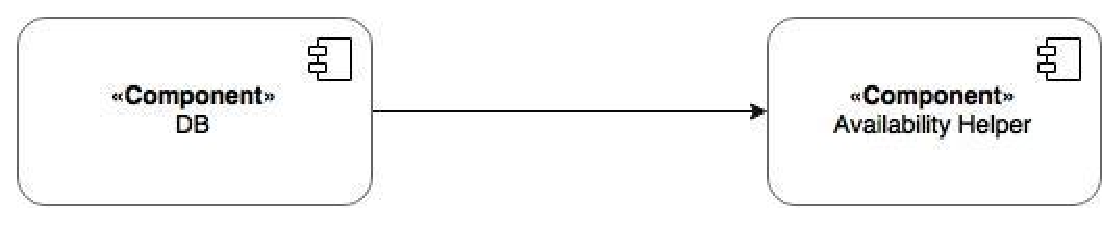
\includegraphics[height=1.4cm,keepaspectratio]{figures/itp1.eps}
	\label{fig:itp1}
\end{figure}

Then the same procedure is followed by replacing the selection controller with other components of the controller system in the following sequence: Reservation Controller, Ride controller, Parking Controller, Discount Controller.

\begin{figure}[h]
	\centering
	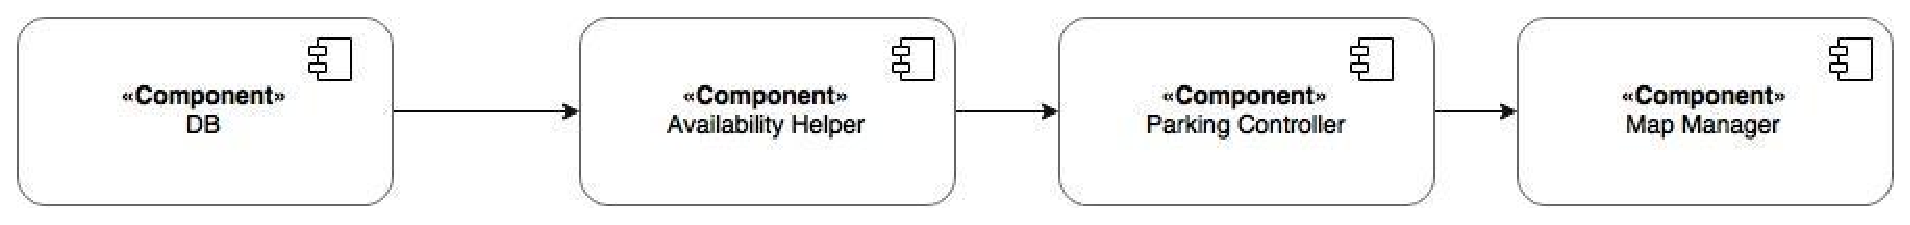
\includegraphics[width=\linewidth,keepaspectratio]{figures/itp6.eps}
	\label{fig:itp6}
\end{figure}

\subsubsection*{Map Manager System}
Generally the communication between the controllers happens through the Map Manager. So, the Map Manager has to be integrated with the Controllers for their communication and also for interaction of the Client with the system.

\begin{figure}[h]
	\centering
	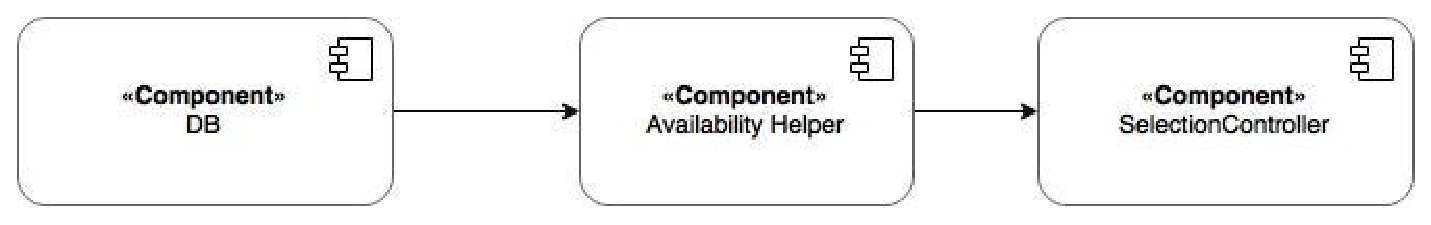
\includegraphics[height=1.4cm,keepaspectratio]{figures/itp2.eps}
	\label{fig:itp2}
\end{figure}

\begin{figure}[h]
	\centering
	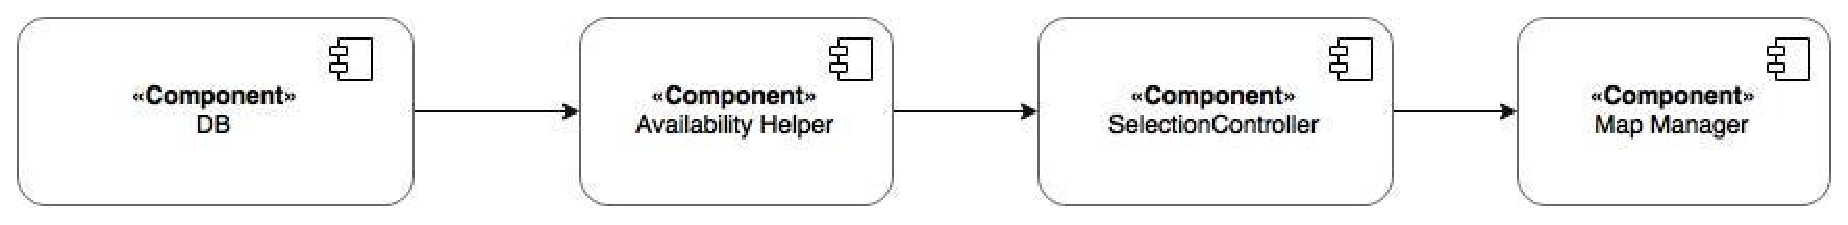
\includegraphics[height=1.4cm,keepaspectratio]{figures/itp3.eps}
	\label{fig:itp3}
\end{figure}

\subsubsection*{Notification System}
The next integration test is executed with the notification system. This notification system is developed by the third party and we just integrate and test here the functionalities. For example: after reserving a car, the user is notified with a confirmation acknowledgement.

\begin{figure}[h]
	\centering
	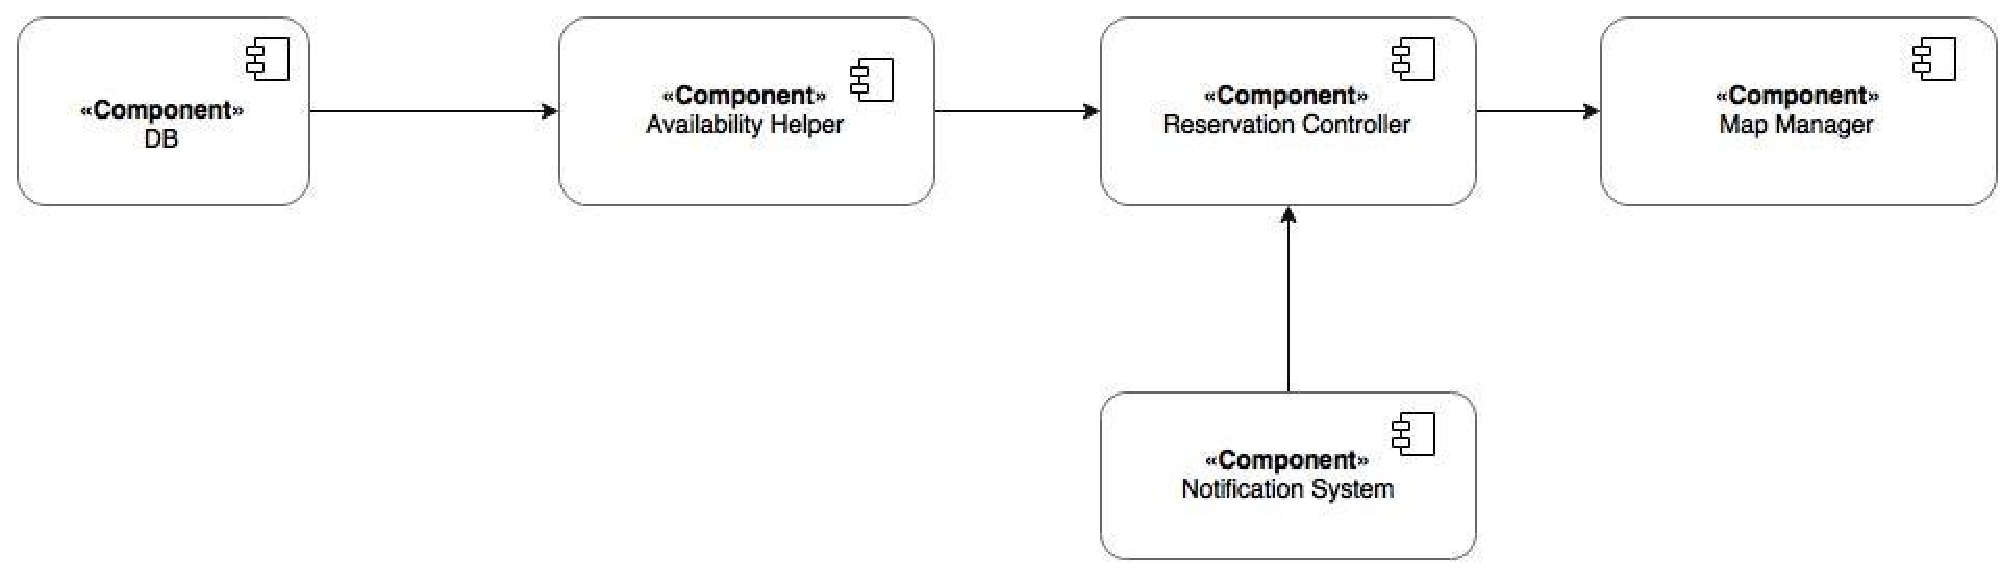
\includegraphics[width=\linewidth,keepaspectratio]{figures/itp4.eps}
	\label{fig:itp4}
\end{figure}

\begin{figure}[h]
	\centering
	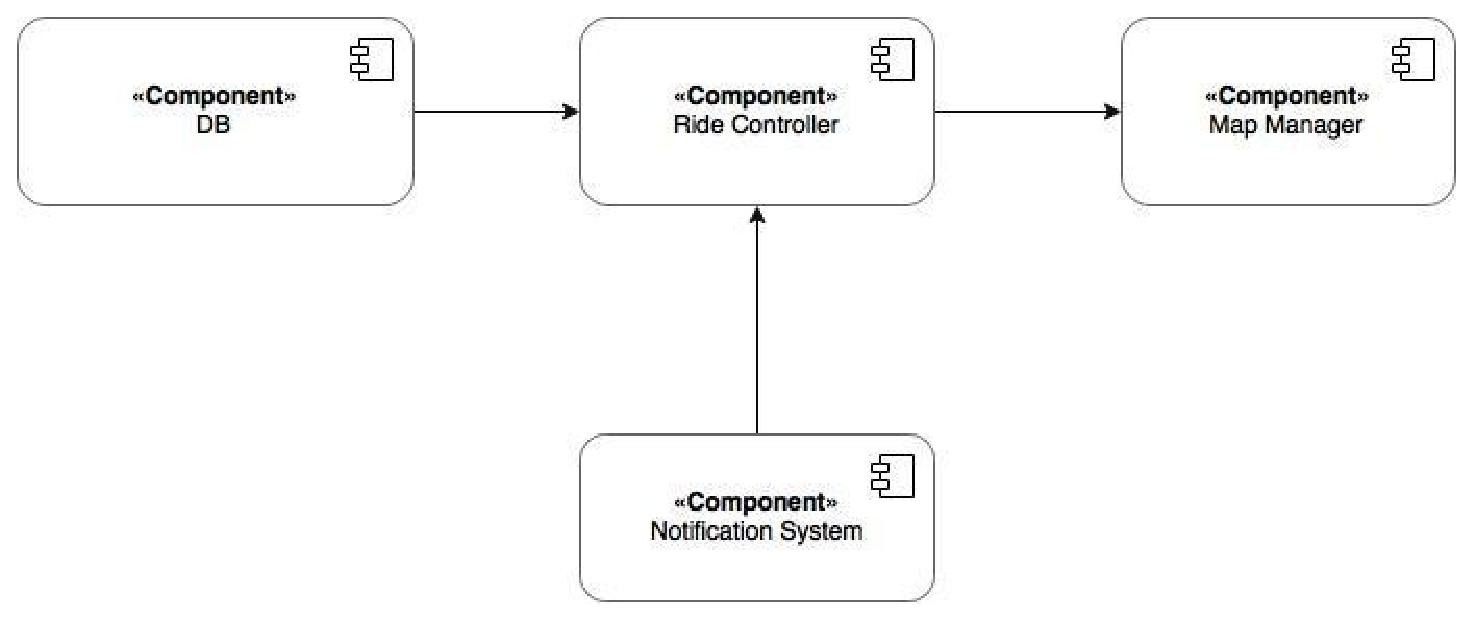
\includegraphics[height=4cm,keepaspectratio]{figures/itp5.eps}
	\label{fig:itp5}
\end{figure}

\begin{figure}[h]
	\centering
	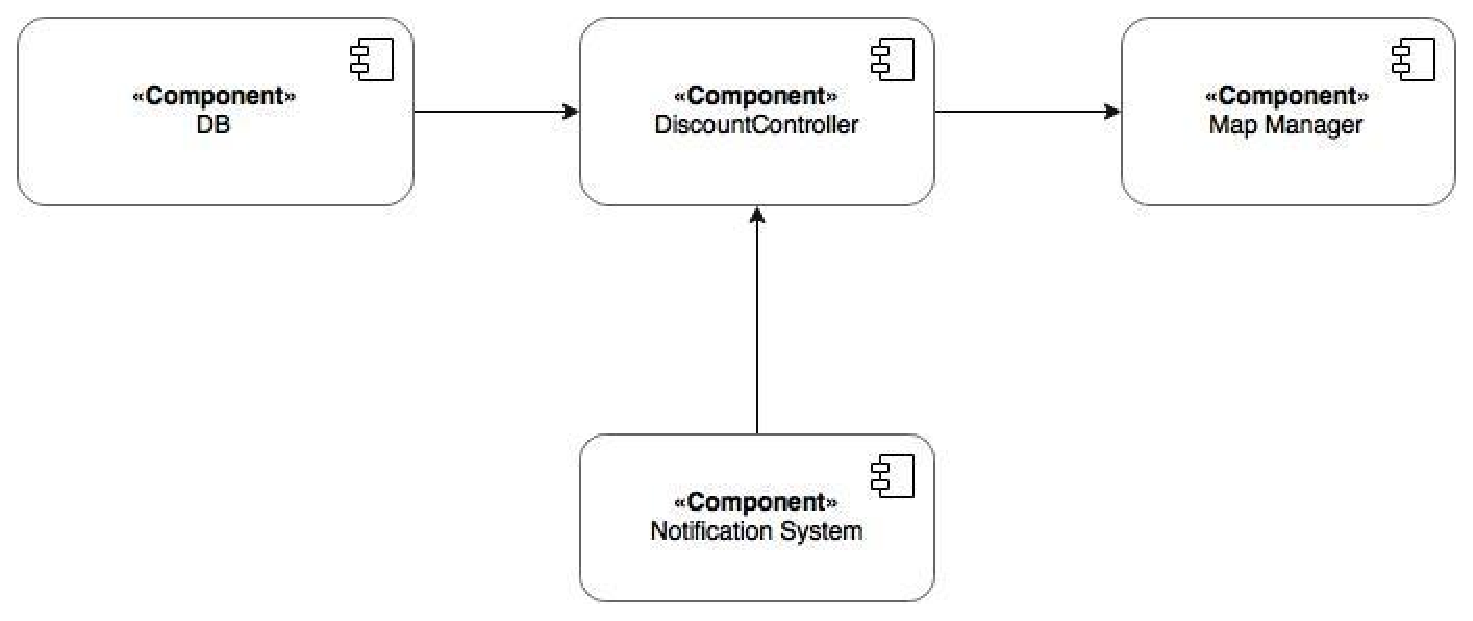
\includegraphics[height=4cm,keepaspectratio]{figures/itp7.eps}
	\label{fig:itp7}
\end{figure}

\newpage
\begin{figure}[h]
	\centering
	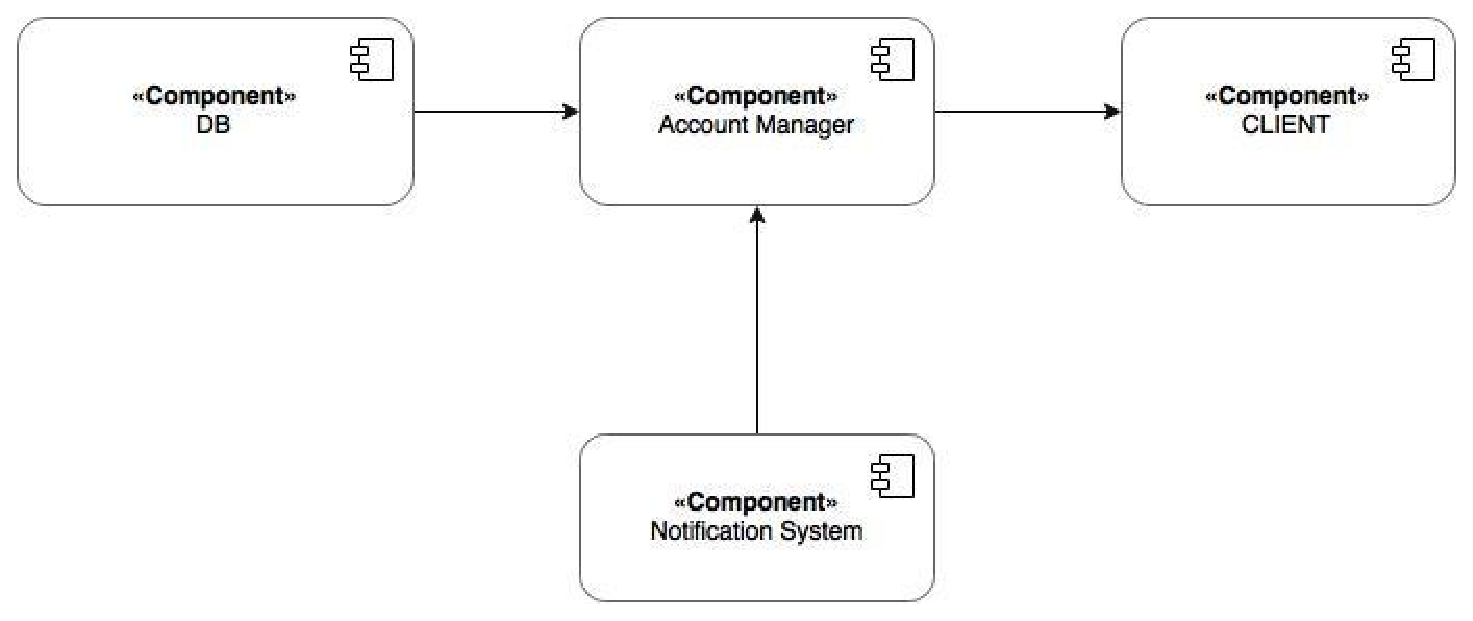
\includegraphics[height=4cm,keepaspectratio]{figures/itp8.eps}
	\label{fig:itp8}
\end{figure}

\begin{figure}[h]
	\centering
	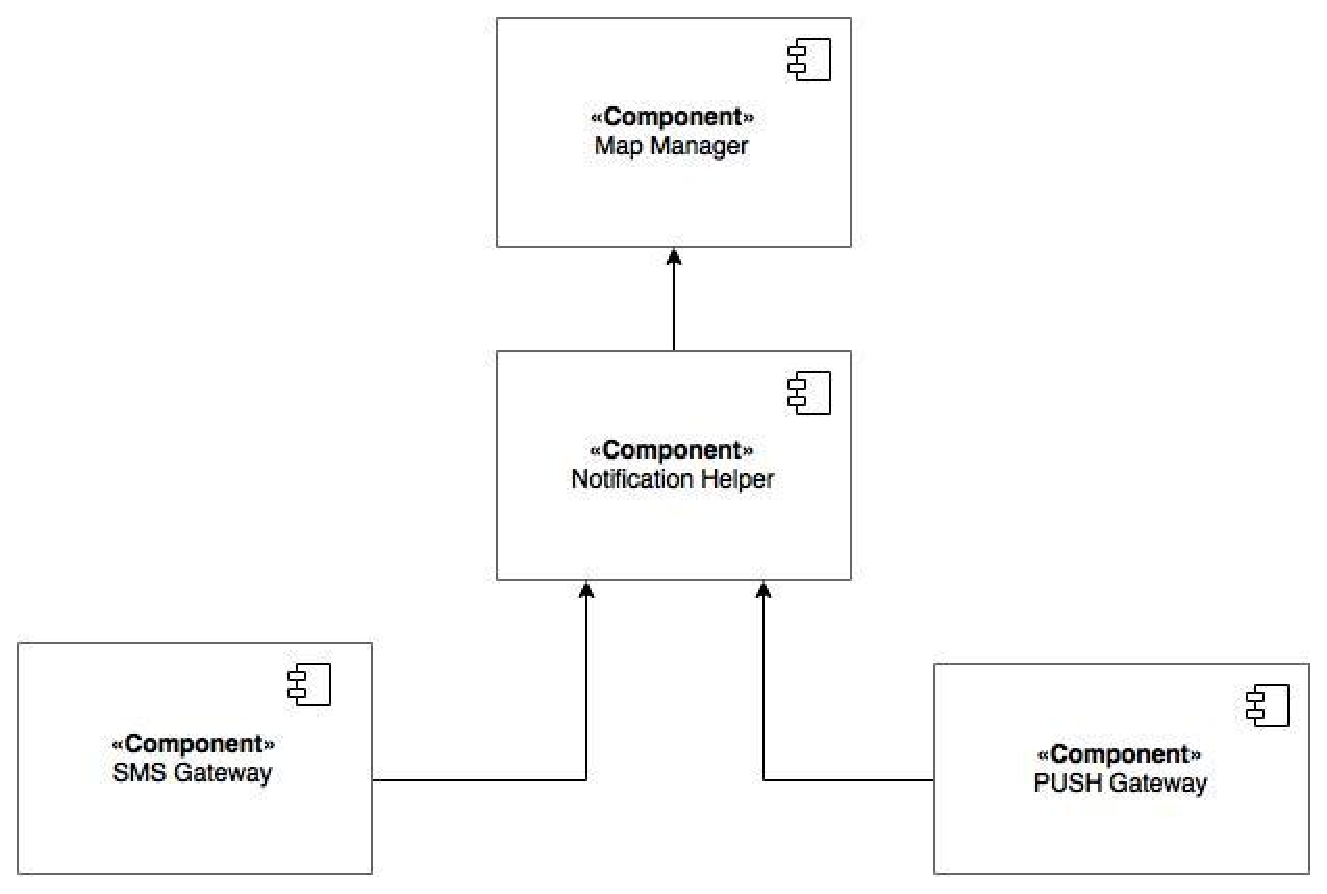
\includegraphics[height=6.285cm,keepaspectratio]{figures/components_notification.eps}
	\label{fig:components_notification}
\end{figure}

\subsubsection*{Payment System}
The payment system is same like the notification system as it is developed by the third party and we just integrate and test here the functionalities.

\newpage
\begin{figure}[h]
	\centering
	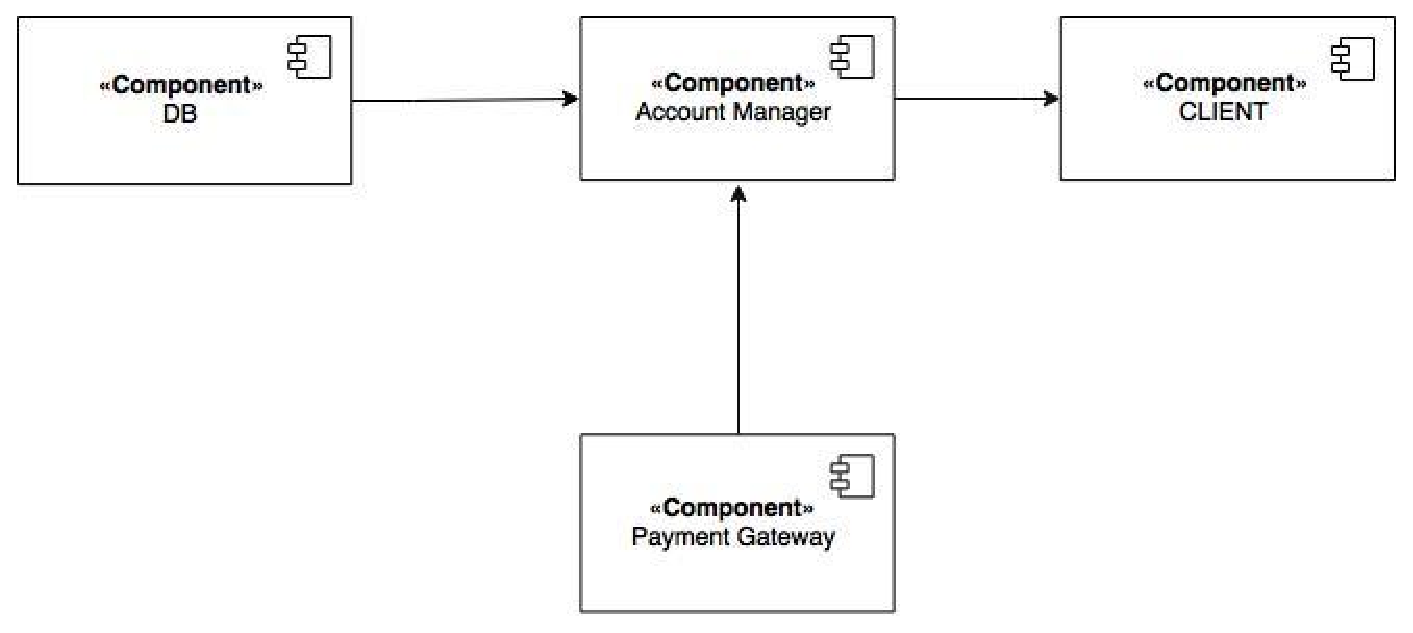
\includegraphics[height=4.38cm,keepaspectratio]{figures/components_payment.eps}
	\label{fig:components_payment}
\end{figure}

\subsubsection*{Account Manager System}
After the integration of the above systems, the account manager is integrated and tested here. The account manager has information about the user details and allows him/her to edit personal informations, upload documents and other services. 

\begin{figure}[h]
	\centering
	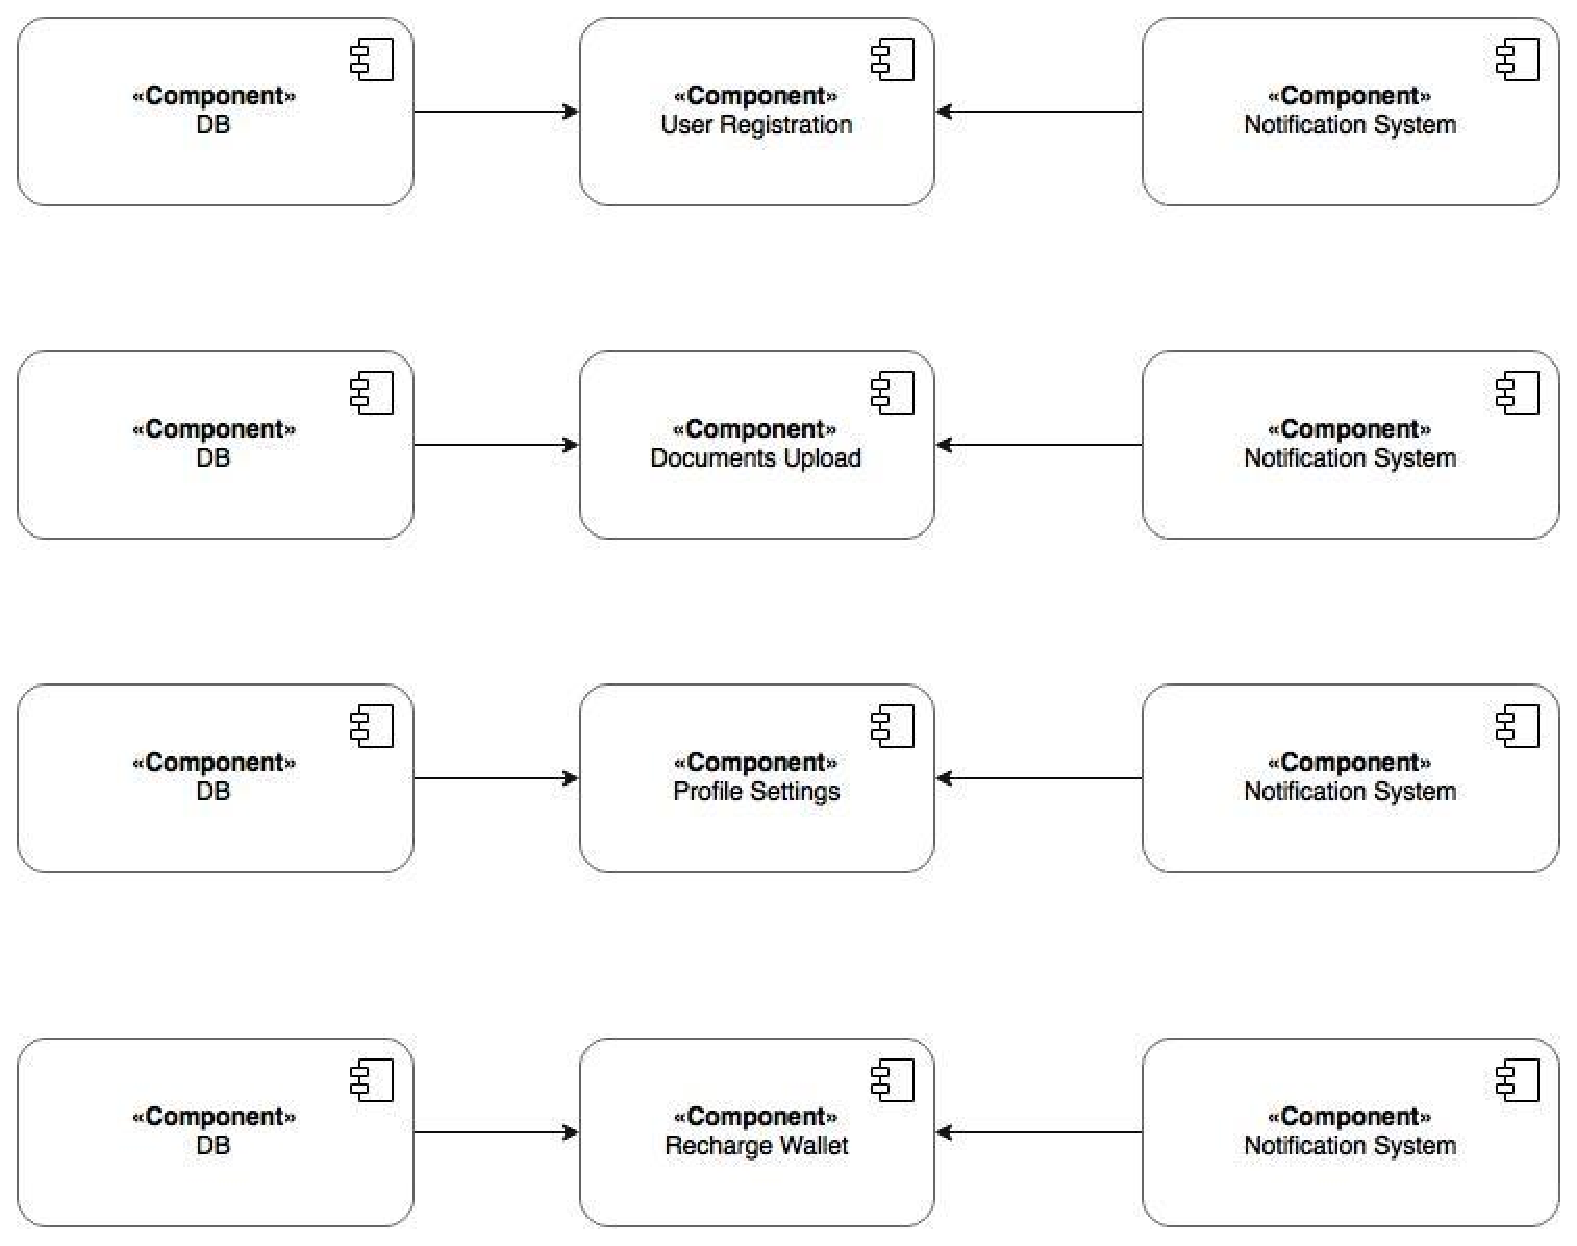
\includegraphics[height=8.86cm,keepaspectratio]{figures/itp9.eps}
	\label{fig:itp9}
\end{figure}

\subsection{Subsystem integration sequence}
Finally test integrate and test the Client system with the overall integrated systems. The high level subsystems are integrated together and the integration architecture of the Power Enjoy service is shown here.

\begin{figure}[h]
	\centering
	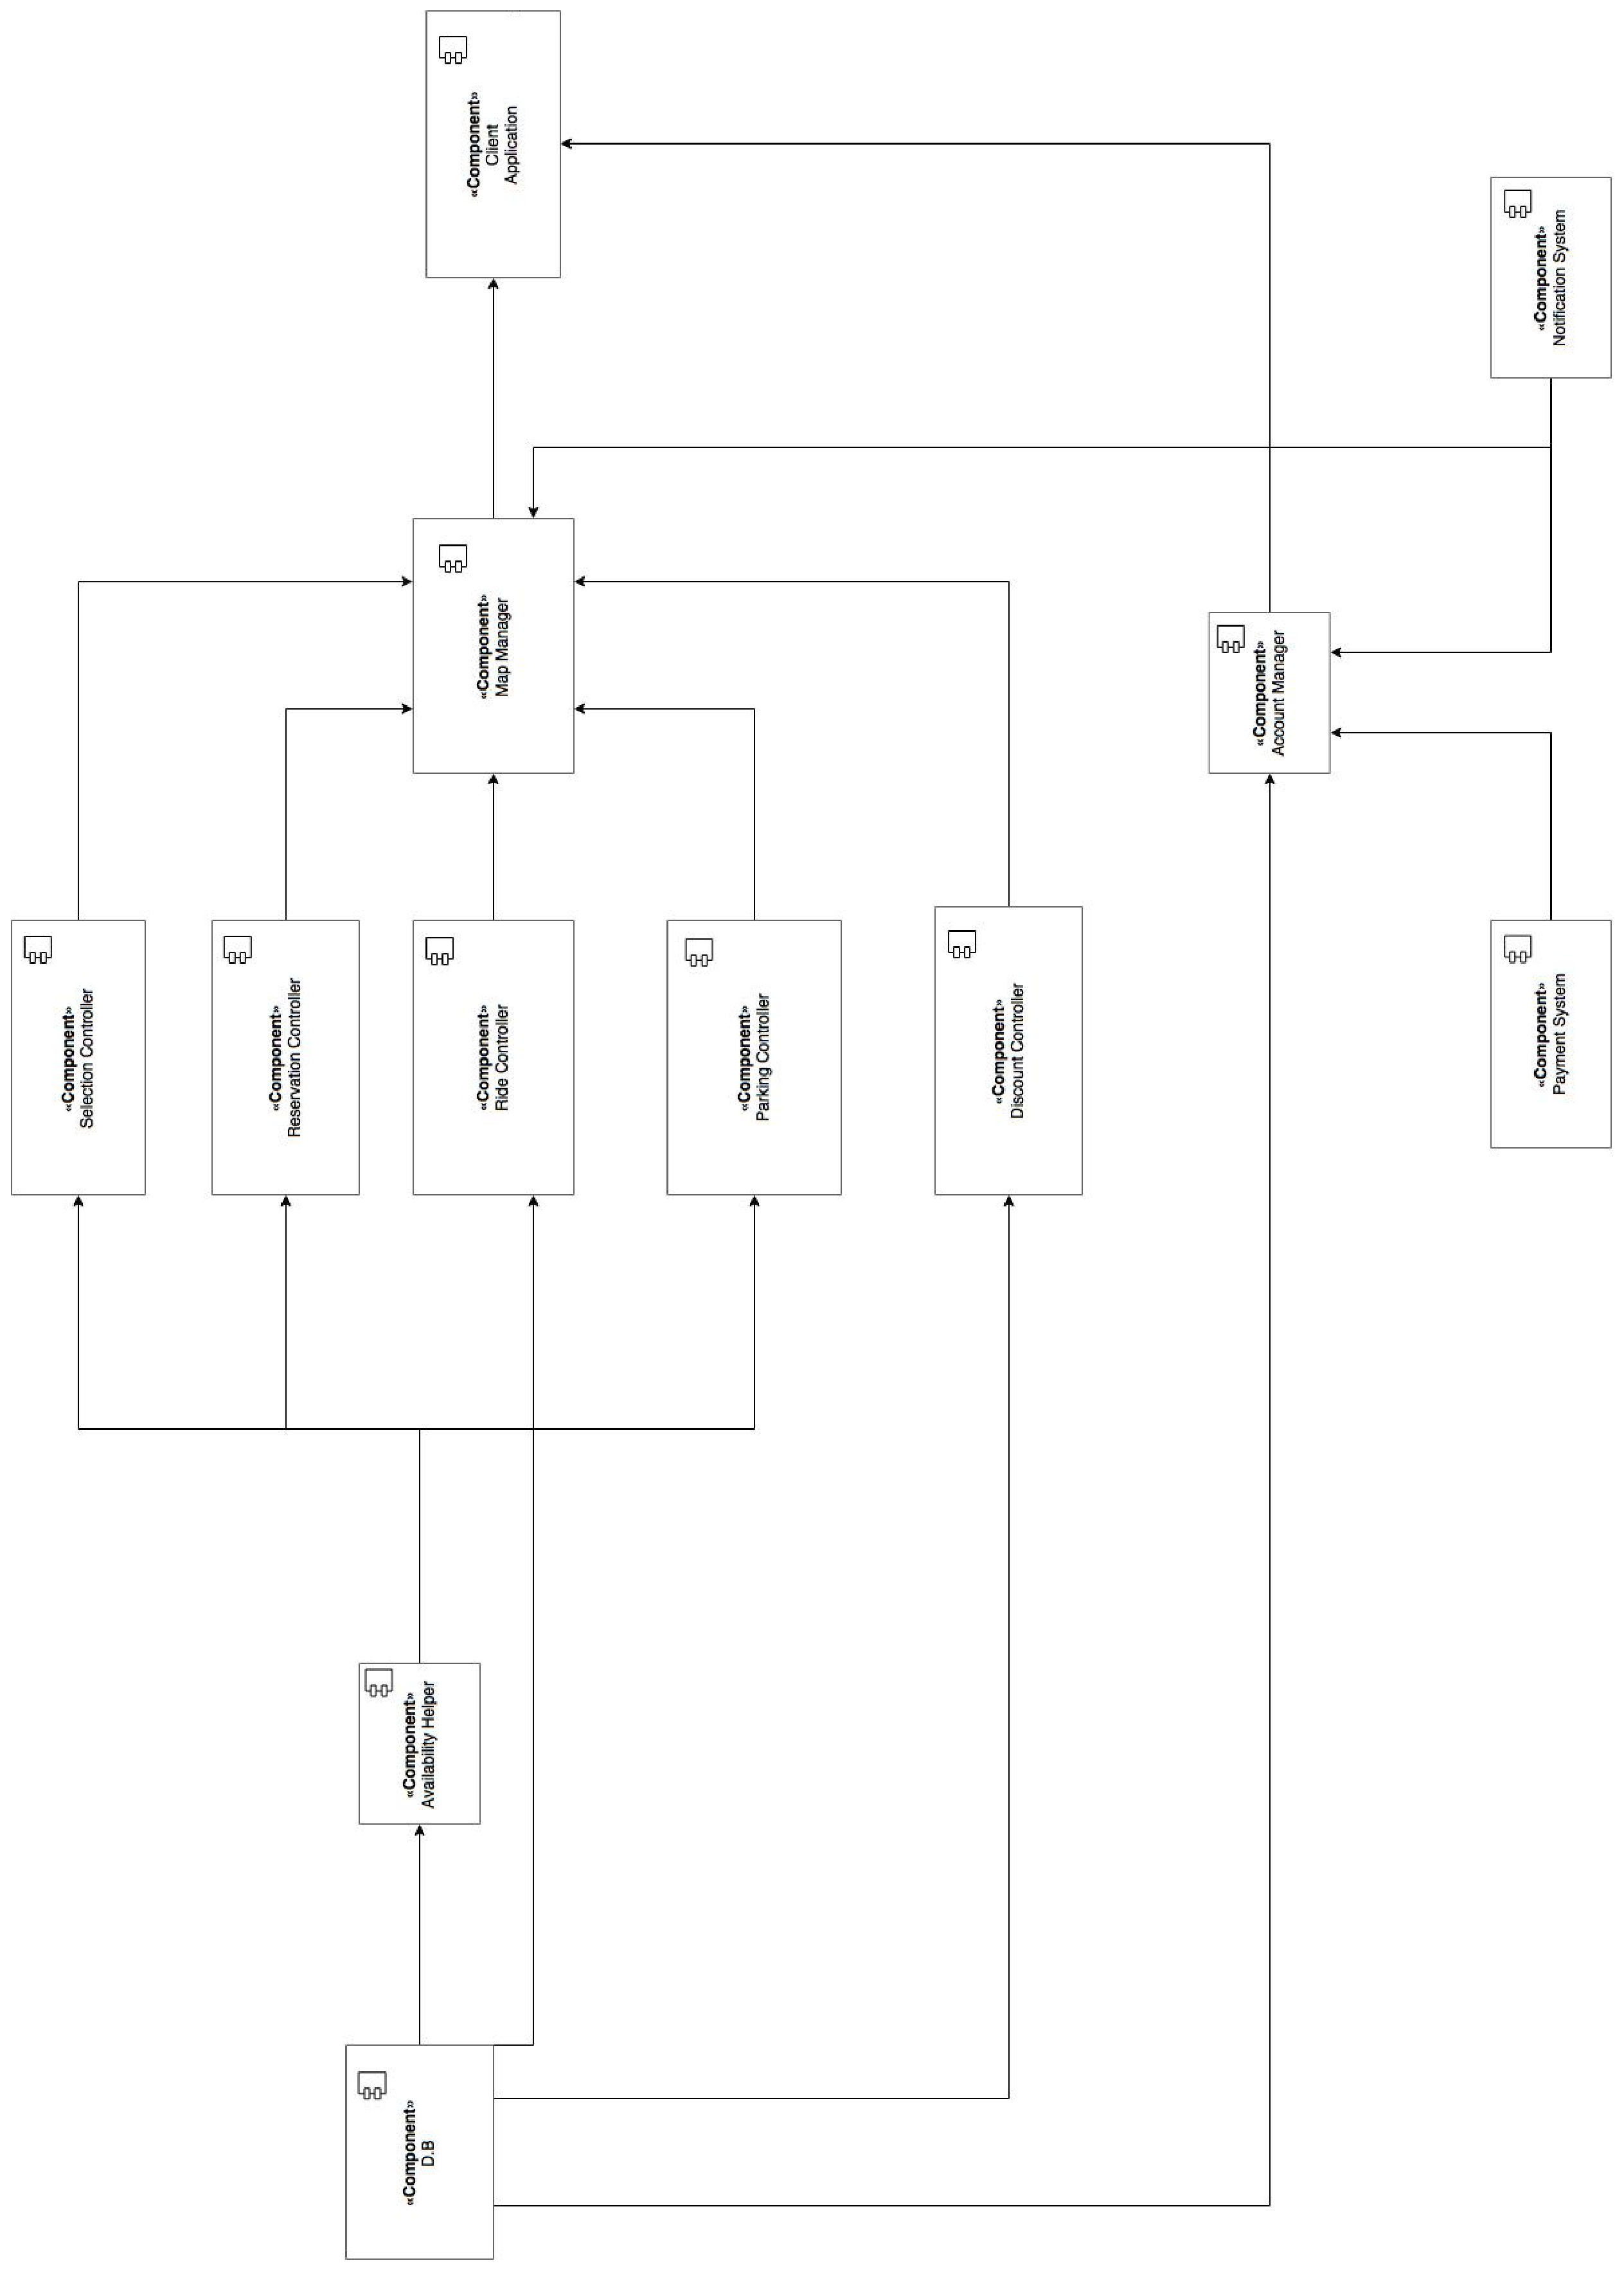
\includegraphics[width=\linewidth,keepaspectratio]{figures/components_controller.eps}
	\label{fig:components_controller}
\end{figure}